\documentclass{article}
\usepackage[UTF8]{ctex}
\usepackage{amsmath}
\usepackage{graphicx}
\usepackage{cite}

\title{龙贝格公式的实现}
\author{21级计算机科学与技术\ 陈岳阳}
\date{\today}

\begin{document}
\maketitle
\tableofcontents

\section{实验目的}

	\subsection{实现四种数值积分方法}
这次试验,我们实现了复化梯形方法、复化Simpson方法、复化Cotes方法和Romberg方法,并在给定积分$\int_1^3e^xdx$和$\int_1^5\frac{1}{1+x}dx$上进行了测试。原要求的误差限为$10^{-6}$,但这样并不能明显的区分四种方法的性能。因此,我们将要求改为$10^{-12}$,以便更加清晰地判断四种方法的性能差异。


\section{实验内容}

	\subsection{四种积分方法的简介}
	
我们即将提到的几种积分方法均假设积分区间是$[a,b]$,被积函数为$f(x)$,步长为h。

假设被积区间为n等分,则$h=\frac{b-a}{n}$。

		\subsubsection{梯形法和Simpson法}

梯形法使用被积函数积分区间在端点处的值进行计算,具有1次代数精度,公式为: $$\int_a^bf(x)dx=\frac{h}{2}[f(a)+f(b)]$$

Simpson法除去积分区间的端点值外,还取用被积函数在积分区间中点的值进行计算。公式为: $$\int_a^bf(x)dx=\frac{h}{6}[f(a)+f(\frac{a+b}{2})+f(a)]$$

		\subsubsection{Cotes公式}

Newton-Cotes公式是一种等距插值型数值积分。节点个数确定时,Cotes系数可通过查表得到。n=4时,Cotes公式为: $$\int_a^bf(x)dx=\frac{b-a}{90}[4f(x_0)+32f(x_1)+12f(x_2)+32f(x_3)+7f(x_4)], x_i=a+i*h$$

Cotes公式的误差为: $$R(f)=\int_a^b\frac{f^{(n+1)}(\xi)}{(n+1)!}w_{n+1}(x)dx=\frac{h^{n+2}}{(n+1)!}\int_0^nf^{(n+1)}(\xi)\Big[\prod\limits_{j=0}^n(t-j)\Big]dt, \xi\in(a,b)$$

当n为偶数时,Cotes公式至少有n+1阶代数精度。

		\subsubsection{复化型求积公式}
复化型求积公式分割积分区间,并在每个区间上进行数值积分,以提高精度。

复化梯形公式: $$\int_a^bf(x)dx=\frac{h}{2}\Big[f(a)+2\sum\limits_{i=1}^{n-1}f(x_i)+f(b)\Big]=T_n$$

余项为$-\frac{b-a}{12}h^2f''(\eta)$\\
\\

复化Simpson公式: $$\int_a^bf(x)dx=\frac{h}{6}\Big[f(a)+4\sum\limits_{i=0}^{n-1}f(x_{i+\frac{1}{2}})+2\sum\limits_{i=1}^{n-1}f(x_i)+f(b)\Big]=S_n$$

余项为$-\frac{b-a}{2880}h^4f^{(4)}(\eta)$\\
\\

复化Cotes公式: $$\int_a^bf(x)dx=\frac{h}{90}\Big[7f(a)+32\sum\limits_{i=0}^{n-1}f(x_{i+\frac{1}{4}})+12\sum\limits_{i=0}^{n-1}f(x_{i+\frac{1}{2}})+32\sum\limits_{i=0}^{n-1}f(x_{i+\frac{3}{4}})+14\sum\limits_{i=1}^{n-1}f(x_i)+7f(b)\Big]=C_n$$

余项为$-\frac{2(b-a)}{945}(\frac{h}{4})^6f^{(6)}(\eta), \eta\in(a,b)$

		\subsubsection{龙贝格公式}

由复化梯形公式,容易得到:$$T_{2n}=\frac{1}{2}T_n+\frac{h}{2}\sum\limits_{k=0}^{n-1}f(x_{k+\frac{1}{2}})$$

分析三种复化方法的误差,可以得到: 
$$
\begin{aligned}
S_n=\frac{4}{3}T_{2n}-\frac{1}{3}T_n\\
C_n=\frac{16}{15}S_{2n}-\frac{1}{15}S_n\\
R_n=\frac{64}{63}C_{2n}-\frac{1}{63}C_n
\end{aligned}
$$

	\subsection{四种积分方法的实现}

受制于篇幅与排版,四种积分方法的代码均于文末及附件中(见Romberg.md)。运行代码需要使用jupyter lab运行Romberg.ipynb。

四种积分方法都有两种形式。一种为<method>,输入积分区间[left,right],区间个数n,函数类型,返回数值积分数值;另一种为<method>\_precision,需要额外输出精度位数和理论值,并打印理论值、数值积分值和达到目标精度时的区间个数。<method>\_precision会调用<method>\_next函数——一个用于递推的函数。其每次将区间个数翻倍。因此,<method>\_precision打印的区间个数一定是2的幂。
\begin{figure}[htbp]
	\centering
	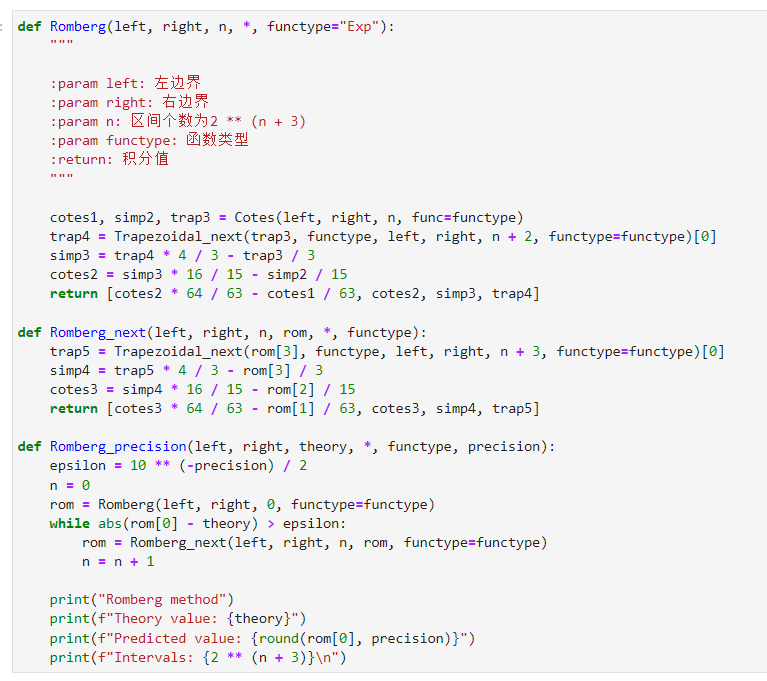
\includegraphics[width=4.8cm, height=3.6cm]{龙贝格1.png}
	\caption{龙贝格公式}
\end{figure}

	\subsection{四种积分方法的测试}

两种测试结果如图所示。可以看出,被积函数、积分区间和误差限相同的情况下,龙贝格算法、Cotes方法、Simpson方法和梯形法的收敛速率依次递减。

\begin{figure}[h]
\begin{minipage}[t]{0.45\linewidth}
\centering
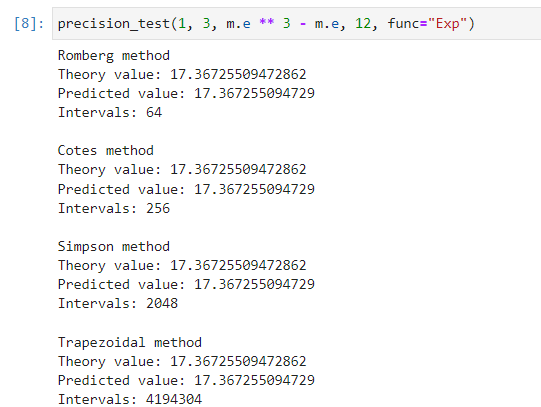
\includegraphics[width=5.5cm,height=3.5cm]{测试图1.png}
\caption{Exp测试}
\end{minipage}
\begin{minipage}[t]{0.45\linewidth}        %图片占用一行宽度的45%
\hspace{2mm}
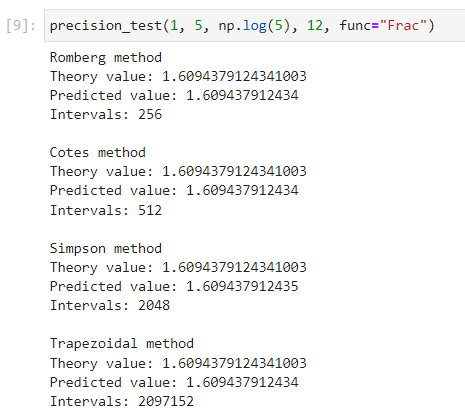
\includegraphics[width=5.5cm,height=3.5cm]{测试图2.png}
\caption{Frac测试}
\end{minipage}
\end{figure}

	\subsection{数值积分在NeRF中的应用}

\begin{figure}[htbp]
	\centering
	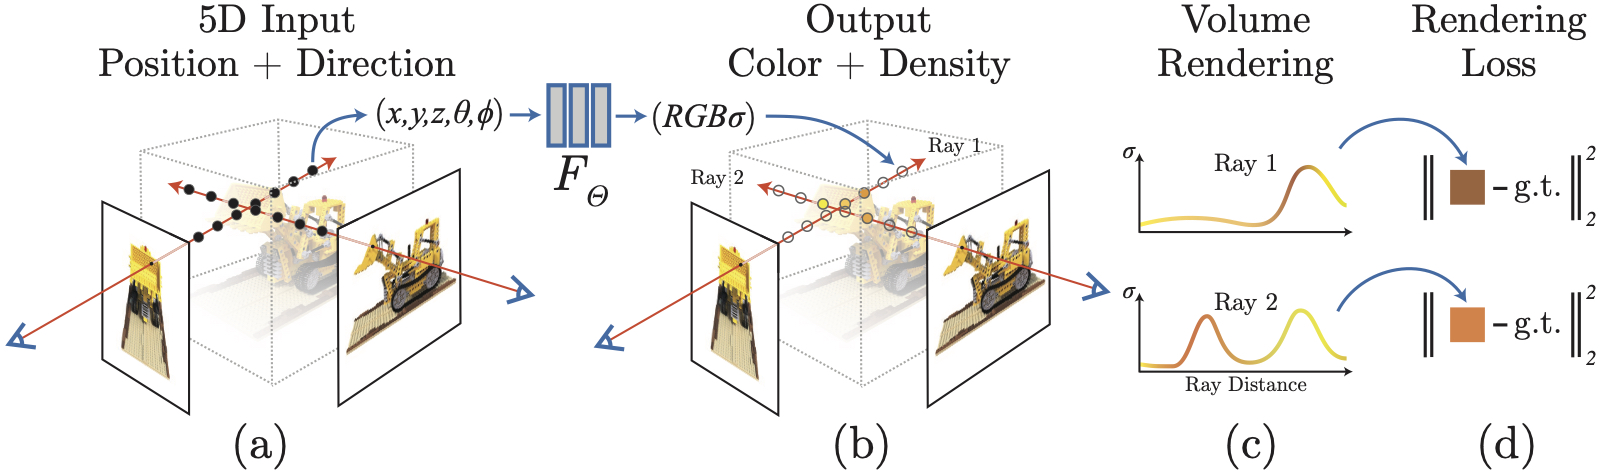
\includegraphics[width=7cm, height=2.5cm]{pipeline.jpg}
	\caption{Pipeline of NeRF}
\end{figure}

NeRF(Neural Radiance Fields)是一种隐式三维场景表示。其将场景表现为空间中任何点的$density\ \sigma$和$color\ c$。

其中,$density\ \sigma(x)$代表ray在x处终止的微分概率。对于有近边界$t_n$,远边界$t_f$的ray $r(t)=o+td$的颜色C(r)是

$$
C(r)=\int_{t_n}^{t_f}T(t)\sigma(r(t))c(r(t),d)dt
$$

T(t)表示沿光线从$t_n$到t的累计透射率,也就是光线从$t_n$传播到t而没有碰到任何其他粒子的概率

$$
T(t)=exp(-\int_{t_n}^t\sigma(r(s))ds)
$$

均匀划分区间,并在每个interval中按均匀分布随机选取一个点。

$$
t_i\sim u\Big[t_n+\frac{i-1}{N}(t_f-t_n),t_n+\frac{i}{N}(t_f-t_n)\Big]
$$

然后使用采样点对$C(r)$进行估计。

$$
C(r)=\sum\limits_{i=1}^{N}T_i(1-exp(-\sigma_i\delta_i))c_i, where\ T_i=exp\Big(-\sum\limits_{j=1}^{i-1}\sigma_j\delta_j\Big),\ \delta_i=t_i-t_{i-1}
$$

由于我们的设备性能有限,在实现了代码后,仍然无法在实验课前完整运行程序一次,无法进行相应演示,只能给出一张tiny\_nerf的结果图片。tiny\_nerf的render部分代码由我们修改并实现。


\begin{figure}[htbp]
	\centering
	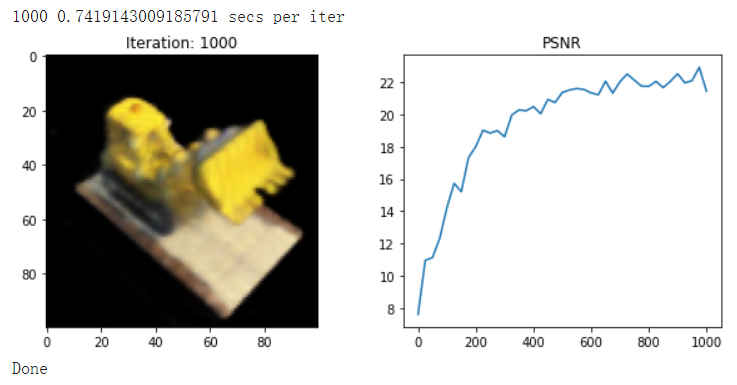
\includegraphics[width=7.5cm, height=4.5cm]{NeRF.png}
	\caption{Tiny NeRF}
\end{figure}

	\subsection{自适应Simpson法}	
		\subsubsection{自适应Simpson法的介绍}
自适应Simpson法是Simpson法的改进。将积分区间等分,并对得到的两个新区间各使用一次Simpson公式,得到的结果的算术平均值与整个区间上进行Simpson公式的结果比较。如果差别较小(通常认为$\delta\leq15\epsilon$),则返回,否则将$\epsilon$减半,并对左右区间递归进行自适应Simpson法。$\epsilon$减半的操作可以保证结果与理论值的误差一定不大于$\epsilon$。

		\subsubsection{自适应Simpson法的实现和测试}
按照介绍,我们可以实现自适应Simpson法。其可以很快的计算出误差在1e-12内的结果。

\begin{figure}[htbp]
	\centering
	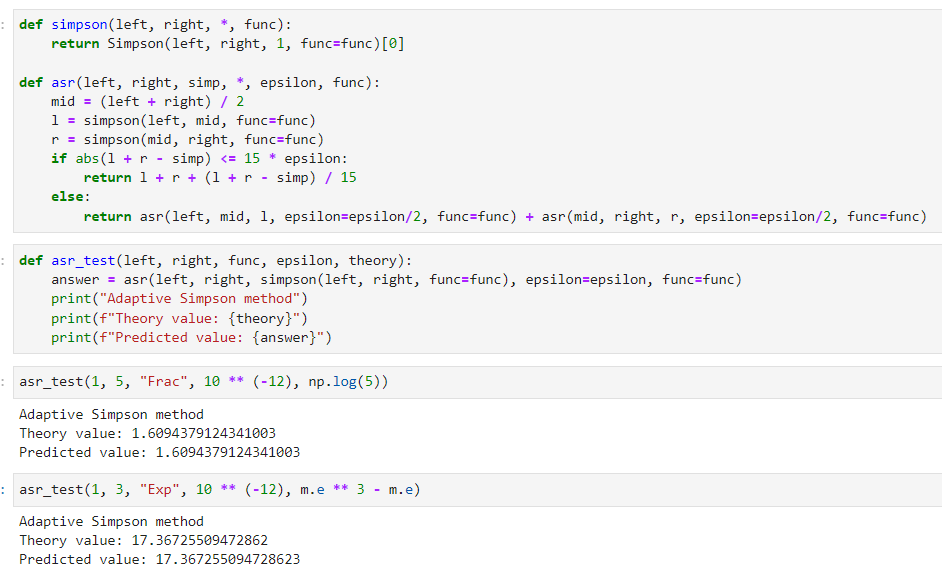
\includegraphics[width=9cm, height=4.5cm]{asr.png}
	\caption{自适应Simpson法}
\end{figure}

	\subsection{实例分析}
由于NeRF的代码无法放出,我们选取了额外的实际问题用于演示。

卫星轨道是一个椭圆,椭圆周长计算公式是
$$
S=4a\int_0^{\frac{\pi}{2}}\sqrt{1-(\frac{c}{a})^2sin^2\theta}d\theta
$$
这里a是椭圆半长轴,c是地球中心与轨道中心的距离。记h为近地点距离,H为远地点距离,R=6371km为地球半径,则
$$
a=(2R+H+h)/2,\ c=(H-h)/2
$$
我国第一颗人造卫星近地点距离h=439km,远地点距离H=2384km,试求卫星轨道的周长。

解:显然,这是个没有解析解的椭圆积分。我们使用自适应Simpson法解出该题。
\begin{figure}[htbp]
	\centering
	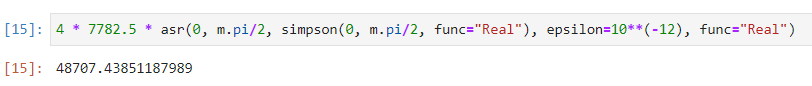
\includegraphics[width=12cm, height=3cm]{realtest.png}
	\caption{实例}
\end{figure}
\section{实验总结}

这次实验,我们实现了四种数值积分方法,比较了它们的性能。相较于其它公式,龙贝格公式有着更快的收敛速度,是一种非常优秀的算法。

此外,NeRF是当前大热的CV技术。数值积分在NeRF上也有一定的应用。在现实中,数值积分也有很大的应用。其用处可见一斑。

实验的过程中,我的代码能力加强了许多,对数值积分的理解更加深入,受益良多。

\section{代码实现}
\end{document}